% !TeX root = POSTER.tex
\documentclass[25pt, a0paper,
portrait,
% landscape,
margin=2mm, 
innermargin=2mm, 
blockverticalspace=7mm, %distance between upper and lower block
colspace=2mm, %distance between left and right block 
subcolspace=0mm]{tikzposter}
		
% -- Packages --------------------------------------------------------%
\usepackage{amsfonts,amssymb,amsmath,mathtools}
\usepackage{defcmlfont}
\usepackage{tikz,lipsum}
\usetikzlibrary{positioning}
\usepackage{float}                           % for minipages at Polarization part
\usepackage{caption}                         % no "Figure" in caption
\captionsetup[figure]{labelformat=empty}

\usepackage{psfrag}

% Load figures command: \inputfig [htb]{fig_dir}{fig_label}
\newcommand*{\inputfig}[3][htb]{{
    \def\fps@figure{#1}
    \def\DIR{#2}
    \def\LABEL{#3}
    \graphicspath{{\DIR/}}
    \psfrag{sm}[c][c]{\small \textsc{Scan me}}


\includegraphics[width=0.03\textwidth]{QRcode_ACoM.eps}
}}

\usepackage{fontawesome}
\usepackage{bm}
\usepackage{bigints}
\usepackage{relsize}

\usepackage{accents}

\usepackage{lipsum} 

\usepackage{babel}
\usepackage{hyperref}
\usepackage{cleveref}

% -- Commands --------------------------------------------------------%
% \newcommand{\wall}{\text{w}}
% \newcommand{\interf}{\text{i}}
% \newcommand{\phase}{k}	
% \newcommand{\liquid}{\ell}
% \newcommand{\steam}{g}
% \newcommand{\out}{\text{out}}
% \newcommand{\tr}{{\mathsf T}}
\newcommand{\WAsigma}{\prescript{\prescript{\mathcal{W}}{}{\!\!\!\mathcal{A}}}{}{\!\sigma}}
\newcommand{\WABsigma}{\prescript{\prescript{\mathcal{W}}{}{\!\!\!\mathcal{A}}}{}{\!\boldsymbol{\sigma}}}

% Mathematic sets
\newcommand{\mbR}{\mathbb{R}}
\newcommand{\mbC}{\mathbb{C}}

% mathcals
\newcommand{\mcA}{\mathcal{A}}
\newcommand{\mcB}{\mathcal{B}}
\newcommand{\mcC}{\mathcal{C}}
\newcommand{\mcD}{\mathcal{D}}
\newcommand{\mcE}{\mathcal{E}}
\newcommand{\mcO}{\mathcal{O}}
\newcommand{\mcS}{\mathcal{S}}
\newcommand{\mcT}{\mathcal{T}}
\newcommand{\mcV}{\mathcal{V}}
\newcommand{\mcW}{\mathcal{W}}

% -- Title, Author, Institute --------------------------------------------------------%
\title{
\begin{minipage}{0.45\textwidth}
		{\bfseries Next-generation all-solid-state battery}
	% \author{\underline{Tuan Vo}$^{\text{a,b}\,\dagger}$, Claas Hüter$^{\text{b}}$, Stefanie Braun$^{\text{a}}$, Manuel Torrilhon$^{\text{a}}$}
	% {\normalsize \underline{Tuan Vo}$^{\text{a,b}\,\dagger}$, Claas Hüter$^{\text{b}}$, Stefanie Braun$^{\text{a}}$, Manuel Torrilhon$^{\text{a}}$}
\end{minipage}
\hfill
\begin{minipage}{0.42\textwidth}
	% \begin{flushleft}
		
\includegraphics[width=0.99\textwidth]{./floats/logos/rwth_acom_en_cmyk_fzj_gap.eps}
	% \end{flushleft}
\end{minipage}
}
\author{
	\underline{Tuan Vo}$^{\text{a,b}\,\dagger}$, Claas Hüter$^{\text{b}}$, Stefanie Braun$^{\text{a}}$, Manuel Torrilhon$^{\text{a}}$\\
\normalsize vo@acom.rwth-aachen.de}
\author{\underline{Tuan Vo}$^{\text{a,b}\,\dagger}$, Claas Hüter$^{\text{b}}$, Stefanie Braun$^{\text{a}}$, Manuel Torrilhon$^{\text{a}}$}
\institute{\large
$\prescript{a}{}{}$Department of Mathematics, Applied and Computational Mathematics (ACoM), 
RWTH Aachen University, Schinkelstraße 02, 52062 Aachen, Germany\\
$\prescript{b}{}{}$Institute of Energy and Climate Research (IEK-2), 
Forschungszentrum Jülich, Wilhelm-Johnen-Straße, 52428 Jülich, Germany
}

% \titlegraphic{
\includegraphics[height=6cm]{./figs/FZJ_only.pdf} \hfill 
\includegraphics[height=6cm]{./figs/rwth_mathcces_bild_rgb_only.pdf} }
% \titlegraphic{
\includegraphics[width=0.3\textwidth]{./floats/logos/rwth_acom_en_cmyk_siamcse23_fzj_gap.eps}}

\renewcommand{\familydefault}{\sfdefault}

\bibliographystyle{plain}

\newcommand{\newcaption}[2]{\parbox{#1}{\centering{\small \it #2\par}}\normalsize}

% -- Predefined Colors and Themes ---------------------- %
% Choose THEME:  Default, Basic, Rays, Simple, Envelope, Wave, Board, Autumn, Desert,
% Explanation THEME: Default(gray+blueBC), Basic(green light), Rays(blue), 
% Simple(red), Envelope(Bluefancy), Wave(Bluefancy2), Board(Bluelight), Autumn(squarebox+bluebrown), Desert(squarebox+bluebrown2),
\usetheme{Default}

\useblockstyle[titleinnersep=0.7mm]{Default}    % change default parameter for title inner sep
% Choose COLOR STYLE:  Default, Blue, BlueGray, BlueOrange, BlueViolet, DarkBlue, GrayBlue, GrayLightblue, GrayRed, Green, GreenOrange, YellowRed
%\definecolor{main}{HTML}{0080FF}
%\definecolor{sub}{HTML}{8CDBFF}
%\usecolorstyle[colorOne=sub, colorTwo=main]{Default}
     
% ---------------------------------------------------------------------------------------------------------------- %
\begin{document}
% Title block
\maketitle[width=800mm]
% \block{}{
% 	d
% }
% ---------------------------------------------------------------------------------------------------------------- %
\block{\bfseries Mathematical modelling for the next-generation All-solid-state batteries: Nucleation $\text{(SE|SSE)}^{\!(*)}$-interface}{
	\begin{minipage}{0.55\textwidth}
		\textbf{Rechargeable Lithium-ion battery} (LIB)
		stays at the heart of electric vehicles, portable electric devices,
		and energy storage systems \cite{vo2018}. 
		Nowadays, LIBs help human life become more efficient 
		as well as to cope with global environment issues thanks to its zero emission.
		However, conventional LIB (cLIB) is sensible to temperature and pressure, 
		easily prone to flammable and explosive. 
		This is mainly due to \underline{liquid-based electrolyte} found in cLIBs.
		
		\textbf{All-solid-state battery} (ASSB) is, therefore, 
		one of promising candidates to overcome bottlenecks of conventional LIBs. 
		It is because the \underline{solid-state electrolyte} (SSE) in ASSB,
		e.g. SSE made of the highly ionic-conductive polycrystalline LLZO, 
		is highly stable towards temperature and pressure. 
		Nevertheless, metallic Lithium dendrite 
		triggered at (SE|SSE)-interface is the main drawback 
		as these dendritic threads extrapolate into grain boundary network of SSE, 
		causing degradation of ionic conductivity 
		and the likelihood of short-circuit.
		\begin{align*}
			a_{\text{Griffith}}:= a^{*}
			= \arg\min_{a\in\mathbb{R}}
			{
				\bigintsss\!\!\!\!\!\!\bigintsss\!\!\!\!\!\!\bigintsss_{\Omega}
				f(a,\bm{u};\lambda,\mu,\bm{d}\otimes\bm{d}) \, d\Omega
				-
				\bigintsss\!\!\!\!\!\!\bigintsss_{\Gamma}
				f(a;\gamma) \, d\Gamma
			}\Bigg|_{\bm{u}^{(s)}}
		\end{align*}
		\textbf{Next-generation All-solid-state battery} (ng-ASSB)
		should, consequentially, be able to cope with 
		micro-dendritic threads at the (SE|SSE)-interface, 
		and hence, 
		to foresee nucleation points caused by propagations 
		% of 
		% these dendrites, 
		% when possible.	
	\end{minipage}%
	\hfill
	\begin{minipage}{0.35\textwidth}
		% \begin{tabular}{|p{\textwidth}}
		% 	This is second part                                                                              \\
		% 	$f(x) = 2x + 3y$ This line may go all along the end and wrap afterwards to the next as seen here \\
		% 	This is a forced next line by ending the previous line 
		% \end{tabular}
		\inputfig{floats/dendrite_pdirection_battonly}{dendrite_pdirection_battonly}
	\end{minipage}%
	% \begin{columns}
	% 	\column{0.5}
	% 	Goal:
	% 	\begin{align}
	% 		a_{\text{Griffith}} := a^{*} = \arg\min_{a\in\mathbb{R}}{\bigintsss\!\!\!\!\!\!\bigintsss\!\!\!\!\!\!\bigintsss_{\Omega} f(a,\bm{u};\lambda,\mu,\bm{d}\otimes\bm{d}) \, d\Omega - \bigintsss\!\!\!\!\!\!\bigintsss_{\Gamma} f(a;\gamma) \, d\Gamma}\Bigg|_{\bm{u}^{(s)}}
	% 	\end{align}
	% 	where
	% 	\column{0.5}
	% 	abc
	% 	% \begin{center}
	% 	% 	% \fbox{\inputfig{floats/creviceAiryWestergaard_compare}{creviceAiryWestergaard_compare}}
	% 	% 	\inputfig{floats/dendrite_pdirection_battonly}{dendrite_pdirection_battonly}
	% 	% \end{center}
	% 	\textbf{This poster} is aimed to model the nucleation
	% 	by taking into consideration
	% 	\underline{polarization}, \underline{structural tensor}, 
	% 	\underline{locally non-uniform electric field}, and 
	% 	\underline{Griffith analysis}. 
	% 	\begin{align}
	% 		 & \rho\,
	% 		\partial^2_{t^2}
	% 		\bm{u}^{(s)}
	% 		+
	% 		\nabla \cdot
	% 		\Big(
	% 		\accentset{\scriptstyle 4}{\mathbb{C}}^{f^{\mathbb{D}(\Omega)}_{(\lambda,\mu)}}
	% 		:\nabla\Bu^{(s)}
	% 		\Big)
	% 		+
	% 		\rho\nabla V_{e}
	% 		= \textbf{0},                                                                                                                                                                                                                                                               \\
	% 		%--------------------------------
	% 		\text{s.t.}\quad 
	% 		 & a_{\text{Griffith}} := a^{*} = \arg\min_{a\in\mathbb{R}}{\bigintsss\!\!\!\!\!\!\bigintsss\!\!\!\!\!\!\bigintsss_{\Omega} f(a,\bm{u};\lambda,\mu,\bm{d}\otimes\bm{d}) \, d\Omega - \bigintsss\!\!\!\!\!\!\bigintsss_{\Gamma} f(a;\gamma) \, d\Gamma}\Bigg|_{\bm{u}^{(s)}}
	% 	\end{align}
	% 	where
	% \end{columns}
	% \begin{center}
	% 	\inputfig{floats/dendrite_pdirection_battonly_maths}{dendrite_pdirection_battonly_maths}
	% \end{center}
}
% ---------------------------------------------------------------------------------------------------------------- %
\begin{columns}
	% FIRST column
	\column{0.5}
	% ---------------------------------------------------------------------------------------------------------------- %
	\block{Next-generation All-solid-state battery (ng-ASSB)}{
		\textbf{Interface} between solid electrode and solid-state electrolyte (SE|SSE) 
		taking place at space charge layer (SCL) \cite{braun2015}
		found in all-solid-state lithium-ion batteries (ASSLiBs) 
		critically exhibits mechanical and electrochemical instability \cite{hueter2017}. 
		This evidence points directly to the fact that the soft metallic lithium negative electrode 
		is erroneously prone to triggering dendritic by-products of silvery lithium metal, 
		under cycles of electric charge \& discharge \cite{kim2022}.

		Besides, polycrystalline garnet-typed solid-state electrolyte such as LLZO 
		exhibit grain boundaries and various sizes and shapes of grains under microscopic observation.
		Therefore, this type of microstructure distinctively leads to nuance destruction of ceramic-like materials.
		Consequentially, dendritic by-products contribute to degradation of ionic conductivity
		and trace along grain boundaries in SSE. 
		
		This phenomenon, notwithstanding, is predicted, quantified, and controlled based on analysing 
		the multi-scale coupled problem subjected to conditions of Griffith criterion.
		% \begin{center}
		% \fbox{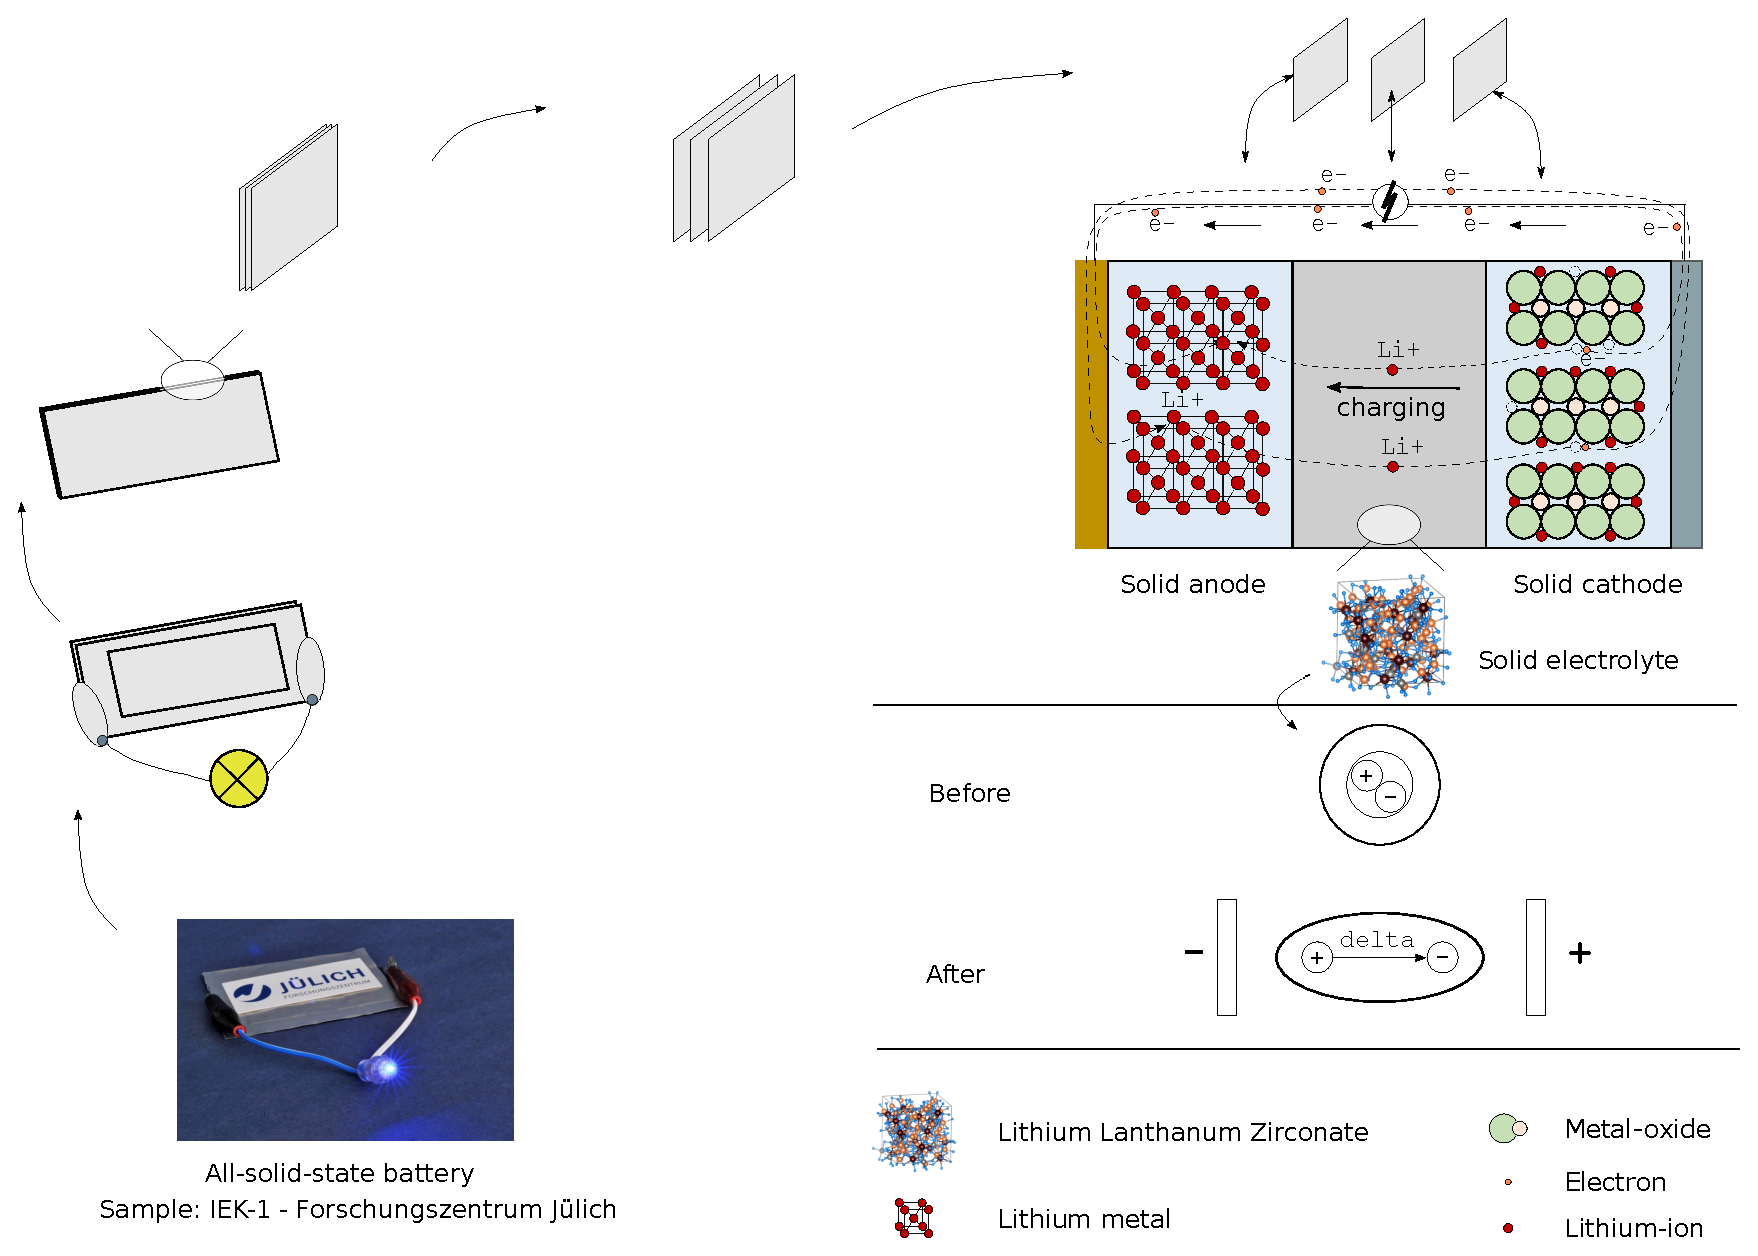
\includegraphics[height=18cm]{./figs/dendrite/dendritetext}}
		% \fbox{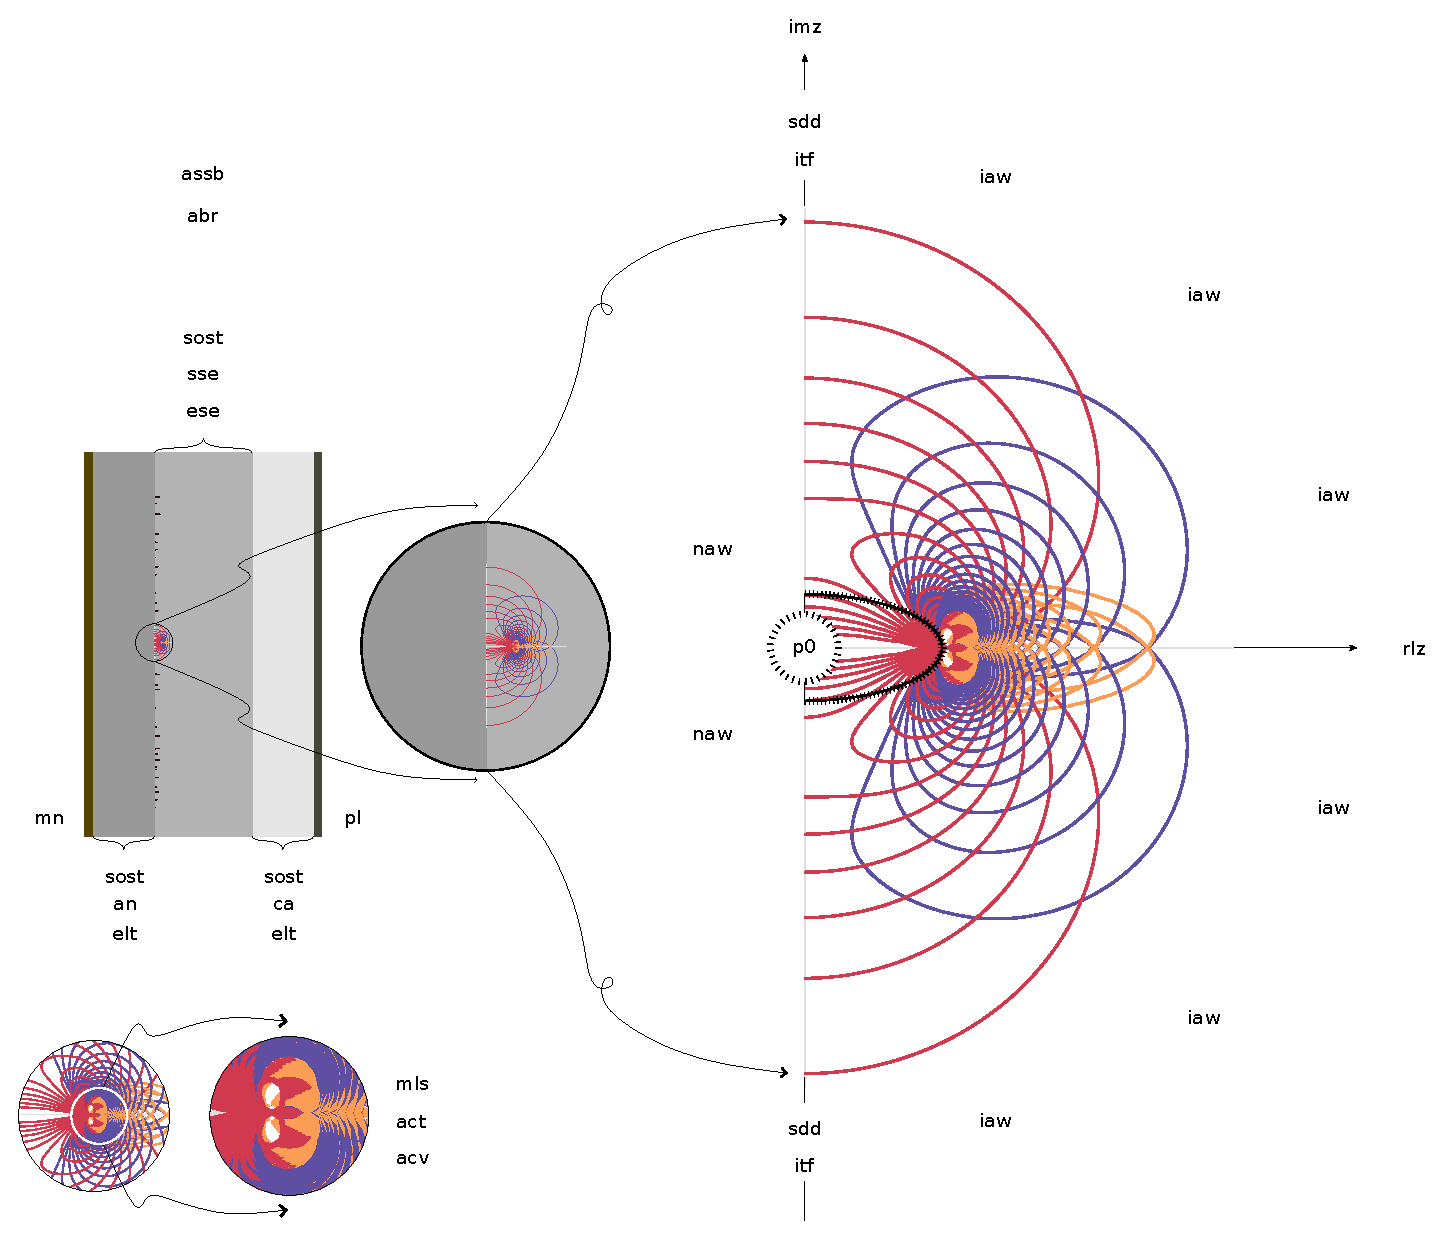
\includegraphics[height=18cm]{./floats/creviceAiryWestergaard_compare/creviceAiryWestergaard_compare.eps}}
		% 	\newcaption{0.8\colwidth}{A sample of a typical all-solid-state battery and its non-scale hierarchical insight into structural layers.}
		% \end{center}
		
		% A typical LIB includes three main components: cathode, anode and electrolyte. 
		% Different types of LIB have a variation of constitutive material composed of battery. 
		% An ASSB means that the three main components are \textbf{all made of solid material}.
	}
	% ---------------------------------------------------------------------------------------------------------------- %
	% \block{Modelling goal: Interface analysis + Numerics}{
	% 	Two main goals to model the solid electrolyte part of the all-solid-state battery is as follows:
	% 	%
	% 	\begin{enumerate}
	% 		\item To capture the \textbf{preferred direction} behaviour of the solid electrolyte due to electric potential.
	% 		\item To satisfy \textbf{thermodynamic consistency}%\cite{braun2015SCL}
	% 		      :
	% 		      \begin{itemize}
	% 			      \item Conservation of mass, linear $\&$ angular momentum and energy for the solid electrolyte.
	% 			      \item Entropy inequality is guaranteed with sharper conditions, which lead to constitutive equation.
	% 		      \end{itemize}
	% 	\end{enumerate}
	% 	\begin{align*}
	% 		a_{\text{Griffith}}:= a^{*}
	% 		= \arg\min_{a\in\mathbb{R}}
	% 		{
	% 			\bigintsss\!\!\!\!\!\!\bigintsss\!\!\!\!\!\!\bigintsss_{\Omega}
	% 			f(a,\bm{u};\lambda,\mu,\bm{d}\otimes\bm{d}) \, d\Omega
	% 			-
	% 			\bigintsss\!\!\!\!\!\!\bigintsss_{\Gamma}
	% 			f(a;\gamma) \, d\Gamma
	% 		}\Bigg|_{\bm{u}^{(s)}}
	% 	\end{align*}
	% }
	% ---------------------------------------------------------------------------------------------------------------- %
	% \block{Continuum physics kinematic}{
	% 	Green-Lagrange strain tensor $\BE$ with respect to \textbf{small} displacement 
	% 	$\partial\Bu/\partial\Bxi = \mathcal{O}(\epsilon), \ \epsilon \ll 1$:
	% 	\begin{align*}
	% 		\BE = \frac{1}{2}(\BF^{\top}\BF -\BI) =\frac{1}{2}\left(
	% 		\frac{\partial\Bu}{\partial\Bxi} + \left( \frac{\partial\Bu}{\partial\Bxi} \right)^{\top}
	% 		+\underbrace{\left( \frac{\partial\Bu}{\partial\Bxi} \right)^{\top}\left( \frac{\partial\Bu}{\partial\Bxi} \right)}_{\text{Neglected}}
	% 		\right) \ \rightarrow \
	% 		\Bvarepsilon := \frac{1}{2}\left(
	% 		\frac{\partial\Bu}{\partial\Bxi} + \left( \frac{\partial\Bu}{\partial\Bxi} \right)^{\top}\right)
	% 	\end{align*}
	% }
	% ---------------------------------------------------------------------------------------------------------------- %	
	% \block{Polarization phenomenon}{
	% 	Due to a source of electric potential pointing from cathode $(+)$ to anode $(-)$ pole, 
	% 	a uniform electric field created has suppressed on 
	% 	the SE occupied between these two poles. Consequently, SE yields to a \textbf{preferred direction}
	% 	under external deformations such as mechanical loading forces.
	% 	% \begin{minipage}{\linewidth}
	% 	% 	\centering
	% 	% 	\begin{minipage}{0.20\linewidth}
	% 	% 		\begin{figure}[H]
	% 	% 			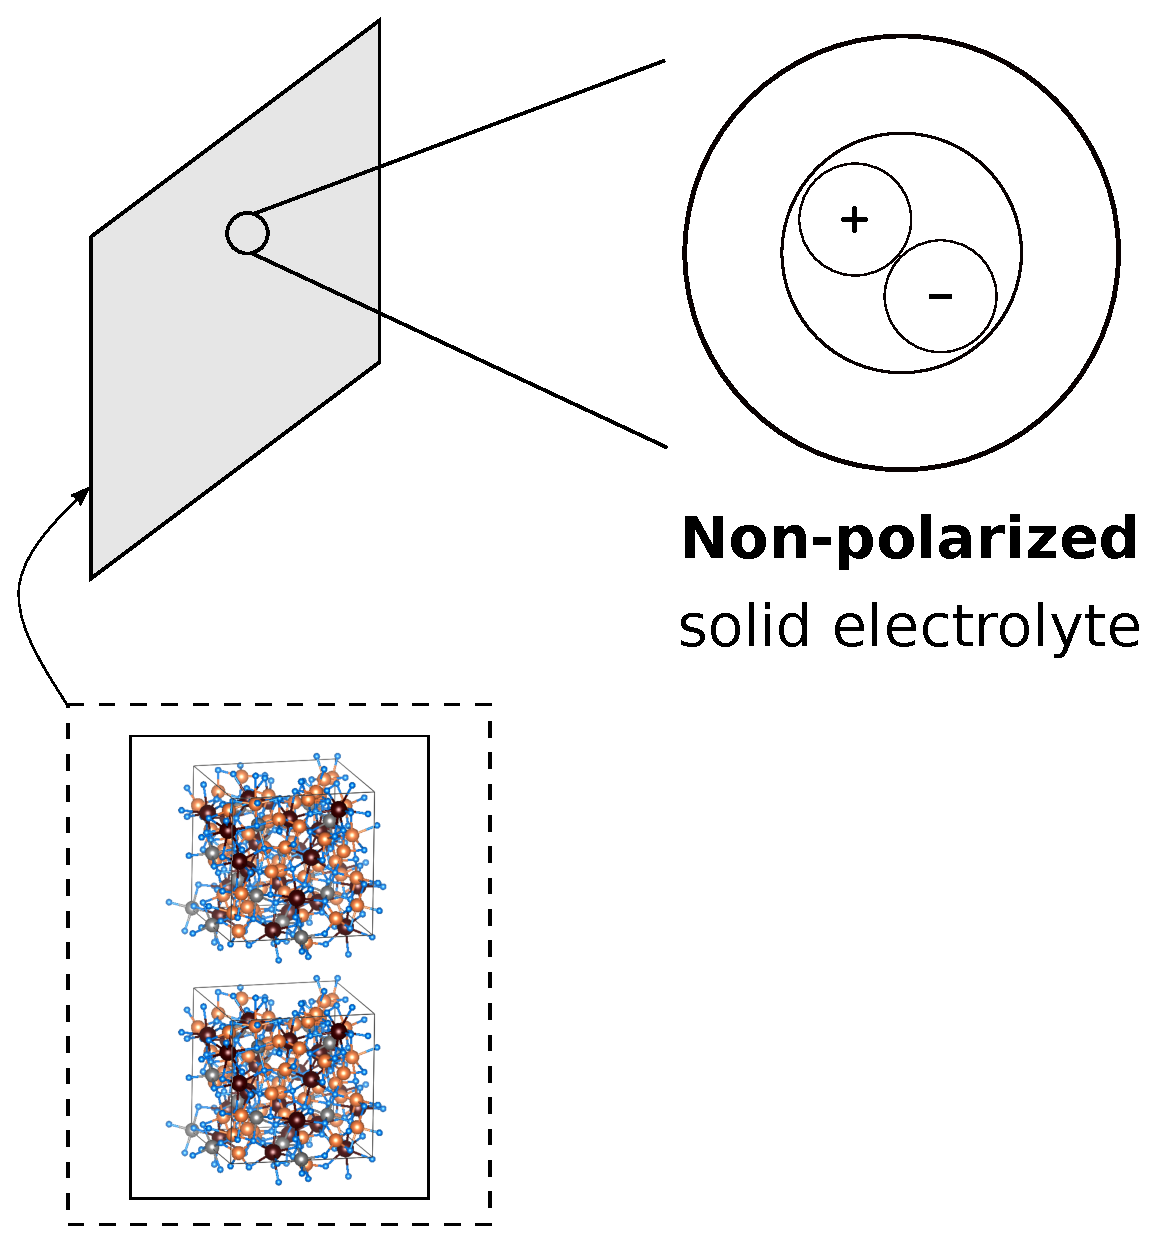
\includegraphics[width=\linewidth]{./figs/polarization/polarizedSEnon}
	% 	% 			%\caption{Non-polarized SE.}
	% 	% 		\end{figure}
	% 	% 	\end{minipage}
	% 	% 	\hspace{0.2\linewidth}
	% 	% 	\begin{minipage}{0.25\linewidth}
	% 	% 		\begin{figure}[H]
	% 	% 			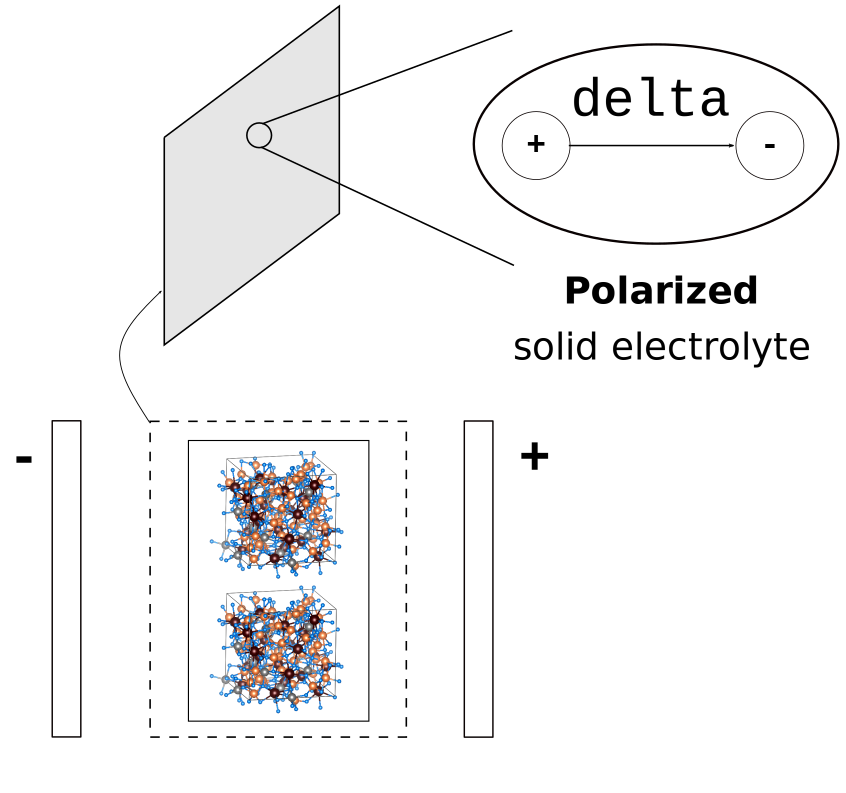
\includegraphics[width=\linewidth]{./figs/polarization/polarizedSE}
	% 	% 			%\caption{Polarized SE.}
	% 	% 		\end{figure}
	% 	% 	\end{minipage}
	% 	% \end{minipage}
	% }
	% ---------------------------------------------------------------------------------------------------------------- %
	% SECOND column
	% ---------------------------------------------------------------------------------------------------------------- %
	\column{0.5}
	\block{Comparison: Analytical vs. Numerical solution}{
		\lipsum[1-2]
		% \begin{center}
		% 	\inputfig{floats/creviceAiryWestergaard_compare}{creviceAiryWestergaard_compare}
		% 	% \inputfig{floats/dendrite_pdirection_battonly}{dendrite_pdirection_battonly}
		% \end{center}
		% \begin{itemize}
		% 	\item Local balance laws governing the infinitesimal elasticity embedded structural tensor:
		% 	      \begin{align*}
		% 		       & \text{Balance of mass}             &  & \dot{\rho} + \rho{\ \rm div}\Bv = 0                             \\
		% 		       & \text{Balance of linear momentum}  &  & \rho\dot{\Bv} = {\rm div}\Bpi + \rho\Bb                         \\
		% 		       & \text{Balance of angular momentum} &  & \Bpi^{\top} = \Bpi                                              \\
		% 		       & \text{Balance of energy}           &  & \rho\dot{e} = \Bpi : \dot{\Bvarepsilon} + \rho r - {\rm div}\Bq
		% 	      \end{align*}
		
		% 	\item Entropy inequality
		% 	      \begin{align*}
		% 		      \rho\calD := \Bpi :\dot{\Bvarepsilon}  -\rho\eta\dot{\theta}- \rho\dot{\Psi} -\frac{1}{\theta}\Bq\cdot\nabla\theta \geq 0 
		% 	      \end{align*}
		
		% 	\item Mathematical model:
		% 	      \begin{align*}
		% 		       & \text{PDE}                   &  & \pi_{ij,j} + \rho b_{i} = 0                                                                                      \\
		% 		       & \text{Kinematic relation}    &  & \varepsilon_{kl} = \frac{1}{2}\left(\frac{\partial u_k}{\partial x_l} + \frac{\partial u_l}{\partial x_k}\right) \\
		% 		       & \text{Constitutive relation} &  & \pi_{ij} = \mathbb{C}_{ijkl}\ \varepsilon_{kl}                                                                   \\
		% 		       & \text{Dirichlet BC}          &  & u_i = \bar{u}_i \text{ on } \partial\Omega_{u_i}                                                                 \\
		% 		       & \text{Neumann BC}            &  & \pi_{ij}n_j = t_i \text{ on } \partial\Omega_{t_i}
		% 	      \end{align*}
		% 	      %
		% 	      \begin{align*}
		% 		      \begin{aligned}
		% 			      \text{where } \qquad 
		% 			      \mathbb{C}_{ijkl} & = \lambda \delta_{ij}\delta_{kl} + 2\mu_T\mathbb{I}_{ijkl}     \\
		% 			                        & + \alpha(\delta_{ij}M_{kl} + M_{ij}\delta_{kl})
		
		% 			      + 2(\mu_L-\mu_T)\left[\mathbb{I}_{\Bd}\right]_{ijkl} + \beta M_{ij}M_{kl}          \\
		% 			      \left[\mathbb{I}_{\Bd}\right]_{ijkl}
		% 			                        & = \frac{1}{2}(d_{i}\delta_{jl}d_{k} + d_{i}\delta_{jk}d_{l}
		
		% 			      +d_{j}\delta_{ik}d_{l} + d_{j}\delta_{il}d_{k})                                    \\
		% 			      \mathbb{I}_{ijkl} & = \frac{1}{2}(\delta_{ik}\delta_{jl} + \delta_{il}\delta_{jk})
		% 		      \end{aligned}
		% 	      \end{align*}
		% \end{itemize}
	}
	% % ---------------------------------------------------------------------------------------------------------------- %	
	% \block{abc}{
	% 	\begin{center}
	% 		% \fbox{\inputfig{floats/creviceAiryWestergaard_compare}{creviceAiryWestergaard_compare}}
	% 		\inputfig{floats/dendrite_pdirection_battonly}{dendrite_pdirection_battonly}
	% 	\end{center}
	% }
	% % ---------------------------------------------------------------------------------------------------------------- %	
	% \block{Structural tensor}{
	% 	SE microstructure with structural tensor $\BM = \Bd \otimes \Bd$ is defined by a symmetry group $\mathbb{G}$:
	% 	\begin{align*}
	% 		\mathbb{G} := \left\{ \BQ_{||_{\Bd}}, \BQ_{\bot_{\Bd}}  \right\} \subset \mathcal{O}(3),
	% 	\end{align*}
	% 	which leads to invariant free energy function $\hat{\Psi}$ under rotations followed by group $\mathbb{G}$:
	% 	\begin{align*}
	% 		\hat{\Psi}(\Bvarepsilon,\BM) = \hat{\Psi}(\BQ\Bvarepsilon\BQ^{\top},\BQ\BM\BQ^{\top}) = \hat{\Psi}(\Bvarepsilon,\BM)  \quad \forall \ \BQ \in \mathbb{G}.
	% 	\end{align*}
	% }
	% % ---------------------------------------------------------------------------------------------------------------- %	
	% \block{Next steps and future direction}{
	% 	\begin{itemize}
	% 		\item Time-dependent implementation, numerical analysis, verification and validation.
	% 		\item Explicit description of coordinate-based polarization variation.
	% 		\item Bridging scale into quantum physics: Update information from quantum for continuum.
	% 		\item Capture a phenomenon so-called \textbf{dendrite formation}:
	% 		    %   \begin{center}
	% 			%       %\vspace*{1em}
	% 			%       \fbox{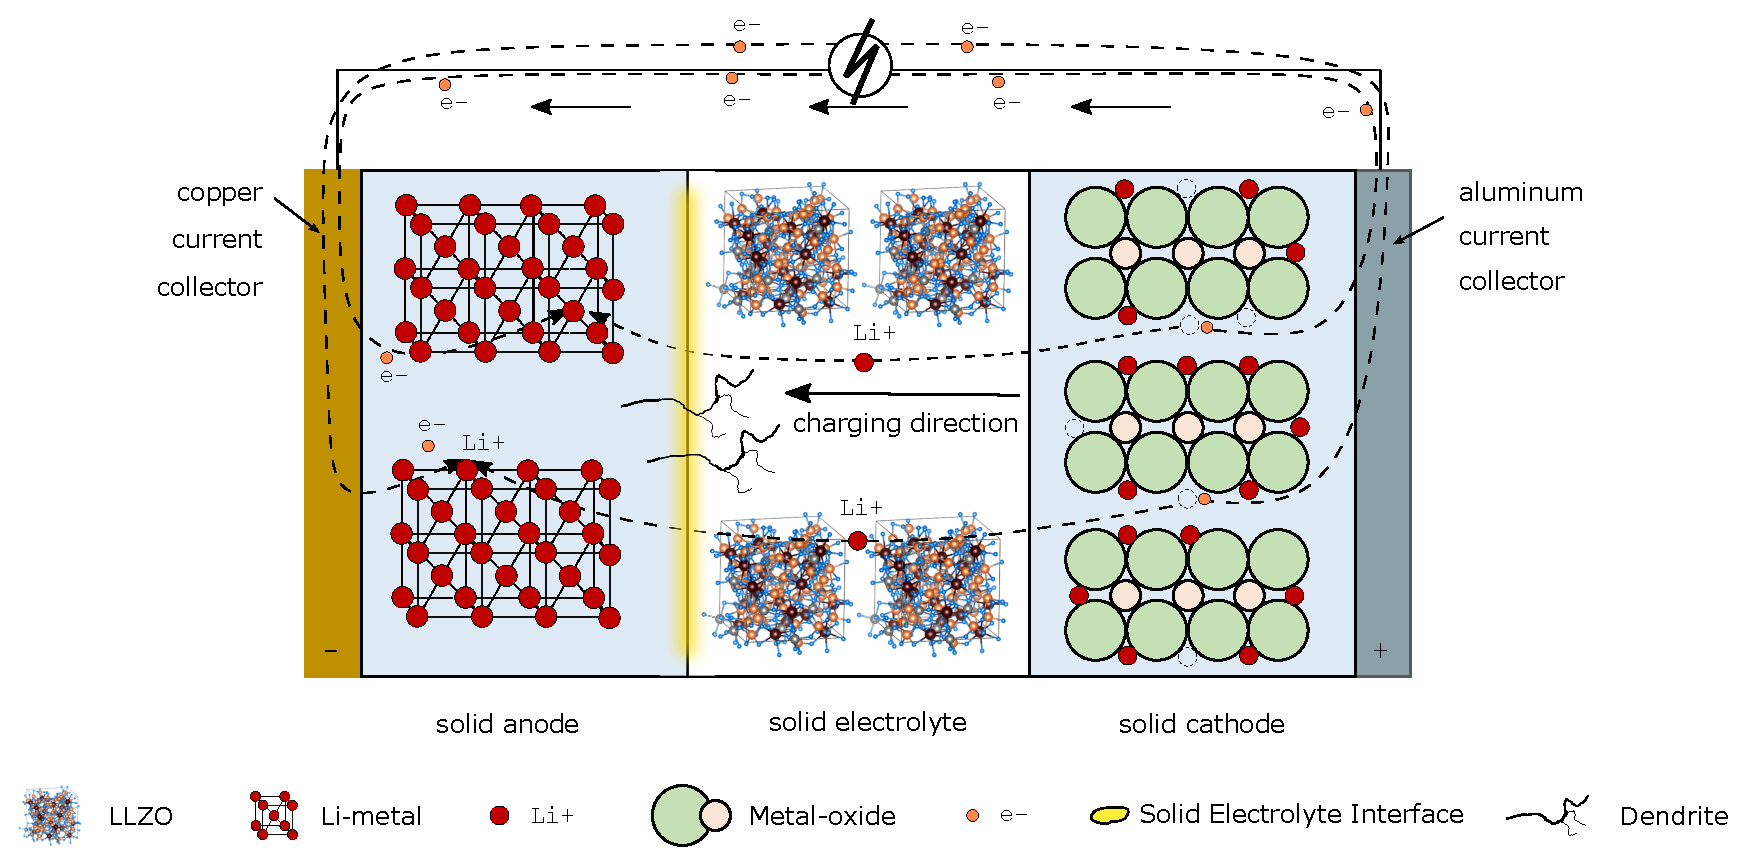
\includegraphics[width=28cm]{./figs/transport/transporttext}}\vspace*{1em}
	% 			%       \newcaption{0.8\colwidth}{Dendrite formation: After a several number of charging cycles, dendrite branches are slowly formed and developed from Solid electrolyte interface (SEI) through grain boundaries.}
	% 		    %   \end{center}
	% 	\end{itemize}
	% }
\end{columns}
% ---------------------------------------------------------------------------------------------------------------- %
\block{Nucleation interface}{
	\begin{minipage}{0.45\textwidth}
		abc
	\end{minipage}
	\hfill
	\begin{minipage}{0.45\textwidth}
		das
	\end{minipage}
	\begin{center}
		\inputfig{floats/routine_woTV}{routine_woTV}
	\end{center}
}

\begin{columns}
	\column{0.15}
	% ---------------------------------------------------------------------------------------------------------------- %	
	\block{Contact}{
		% {
		% 		\raggedleft
		% 		\begin{tikzpicture}
		% 			\node (qrcode) {\inputfig{floats/QRcode_ACoM}{QRcode_ACoM}};
		% 			\node[left= 0mm of qrcode.north west, yshift=-15mm] {Tuan Vo};
		% 			% \node[left= 0mm of qrcode.north west, yshift=-40mm] {Applied and Computational Mathematics (ACoM)};
		% 			% \node[left= 0mm of qrcode.north west, yshift=-55mm] {RWTH Aachen University};
		% 			\node[left= 0mm of qrcode.north west, yshift=-30mm] {vo@acom.rwth-aachen.de};
		% 		\end{tikzpicture}
		% 	}
		\begin{center}
			\inputfig{floats/QRcode_ACoM_Email}{QRcode_ACoM_Email}
		\end{center}
		% \inputfig{floats/QRcode_ACoM}{QRcode_ACoM}
		% Tuan Vo $\cdot$ RWTH Aachen University $\cdot$ Email: vo@acom.rwth-aachen.de
	}
	\column{0.85}
	% % ---------------------------------------------------------------------------------------------------------------- %	
	\block{References}{
		\vspace*{-3em}
		\renewcommand{\refname}{~}
		\begin{thebibliography}{2}
			\bibitem{vo2018}
			\textbf{T.Vo}, \emph{Modeling the swelling phenomena of li-ion batt.
				cells based on a numerical chemo-mech. coupled approach}.
			MA, Robert Bosch Battery Systems GmbH, 2018.
			
			\bibitem{braun2015}
			\textbf{S.Braun},\! C.Yada and A.Latz,\!\!
			\emph{Thermodynamically consistent model for
				Space-Charge-Layer formation in a solid electrolyte}.
			Jr. Phys. Chem.,\! 119,\! 22281-22288, 2015.
			
			\bibitem{hueter2017}
			\textbf{C.Hüter}, S.Fu, M.Finsterbusch, E.Figgemeier, L.Wells, and R.Spatschek,
			\emph{Electrode-electrolyte interface stability in solid state electrolyte system:
				influence of coating thickness under varying residual stresses}. 
			AIMS materials Science, 4(4):867-877, 2017.
			
			\bibitem{kim2022}
			\textbf{S.Kim}, 
			J.S.Kim, L.Miara, Y.Wang, S.K.Jung, S.Y.Park, Z.Song, 
			H.King, M.Badding, J.M.Chang, V.Roev, G.Yoon, R.Kim, J.H.Kim, K.Yoon, D.Im, and K.Kang,
			\emph{High-energy and durable li metal batt. using garnet-type
				solid electrolytes with tailored li-metal compatibility}.
			Nature Communications, 13(1):1883, 2022.
			% $(*)$ (Solid electrode | Solid-state electrolyte)
		\end{thebibliography}
	}
\end{columns}
% ---------------------------------------------------------------------------------------------------------------- %	
% \block{References}{
% 	\vspace*{-3em}
% 	\renewcommand{\refname}{~}
% 	\begin{thebibliography}{2}

% 		\bibitem{viozat1997implicit}
% 		\textbf{T. Vo} \emph{Modeling the swelling phenomena of li-ion battery
% 			cells based on a numerical chemo-mechanical coupled approach}. 
% 		Master thesis, Robert Bosch Batteries Systems GmbH, 2018.

% 		\bibitem{braun2015SCL}
% 		\textbf{S. Braun}, C. Yada and A. Latz. \emph{Thermodynamically consistent model for
% 			Space-Charge-Layer formation in a solid electrolyte}. 
% 		Journal of Physical Chem., 119, 22281-22288, 2015.

% 		\bibitem{hueter2017}
% 		\textbf{C. Hüter}, S. Fu, M. Finsterbusch, E. Figgemeier, L. Wells, and R. Spatschek. 
% 		Electrode-electrolyte interface stability in solid state electrolyte system: 
% 		influence of coating thickness under varying residual stresses. 
% 		AIMS materials Science, 4(4):867-877, 2017.

% 		\bibitem{kim2022}
% 		\textbf{S. Kim}, J. S. Kim, L. Miara, Y. Wang, S. K. Jung, S. Y. Park, Z. Song, 
% 		H. King, M. Badding, J. M. Chang, V. Roev, G. Yoon, R. Kim, J. H. Kim, K. Yoon, D. Im, 
% 		and K. Kang. “High-energy and durable lithium metal batteries using garnet-type 
% 		solid electrolytes with tailored lithium-metal compatibility,” 
% 		Nature Communications, 13(1):1883, Apr 2022.
% 		% $(*)$ (Solid electrode | Solid-state electrolyte)
% 	\end{thebibliography}
% }
\end{document}
% ---------------------------------------------------------------------------------------------------------------- %